\chapter{Boolesk algebra}
\label{chap:ch13}
I kapitel~\ref{chap:ch2} udforskede vi det binære, det decimale, det oktale og det hexadecimale talsystem og lærte at omregne mellem dem og at regne binært. Totalssystemet er med sit grundtal 2 særligt vigtigt i computere, fordi digitale systemer repræsenterer og behandler information ved hjælp af to logiske tilstande.

Når vi går fra at arbejde med binære tal til at forstå \textbf{boolesk algebra}, tager vi det næste skridt i forståelsen af, hvordan computere udfører logiske operationer med binære værdier. Talsystemerne gav os en forståelse af, hvordan tal repræsenteres og behandles. Boolesk algebra gør det muligt at forstå, hvordan beslutninger og logiske processer udføres i digitale systemer. Kort sagt giver boolesk algebra de regler, der styrer logiske beslutninger i det binære system, på samme måde som aritmetikken fungerer i talsystemerne.

\section{Introduktion til boolesk algebra}
Boolesk algebra er en matematisk ramme, der arbejder med binære værdier -- typisk repræsenteret som 0 og 1 -- og viser os, hvilke slags operationer der kan udføres på bit. Systemet blev først introduceret af \textbf{George Boole} i midten af det 19. århundrede. Det danner grundlaget for moderne digital logik og er uundværligt inden for datalogi og elektroteknik.

\begin{figure}[h]
    \centering
    \begin{multicols}{2}  % Split the figure into two columns

        % First image and its caption
        \begin{center}
            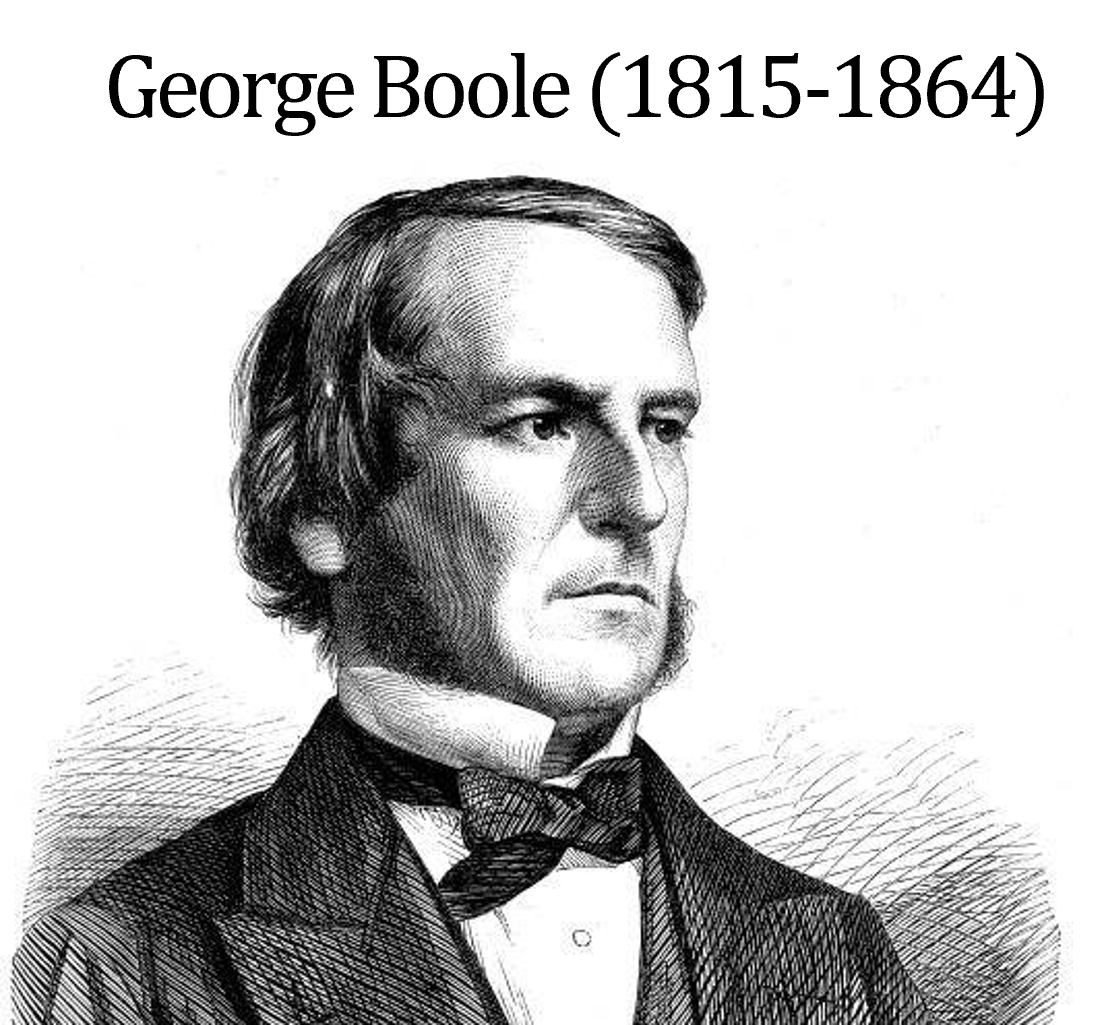
\includegraphics[width=0.6\linewidth]{figure/boole.png}  % Adjust the width as needed
            \caption{Udviklede logikkens regler.}
        \end{center}

        % Second image and its caption
        \begin{center}
            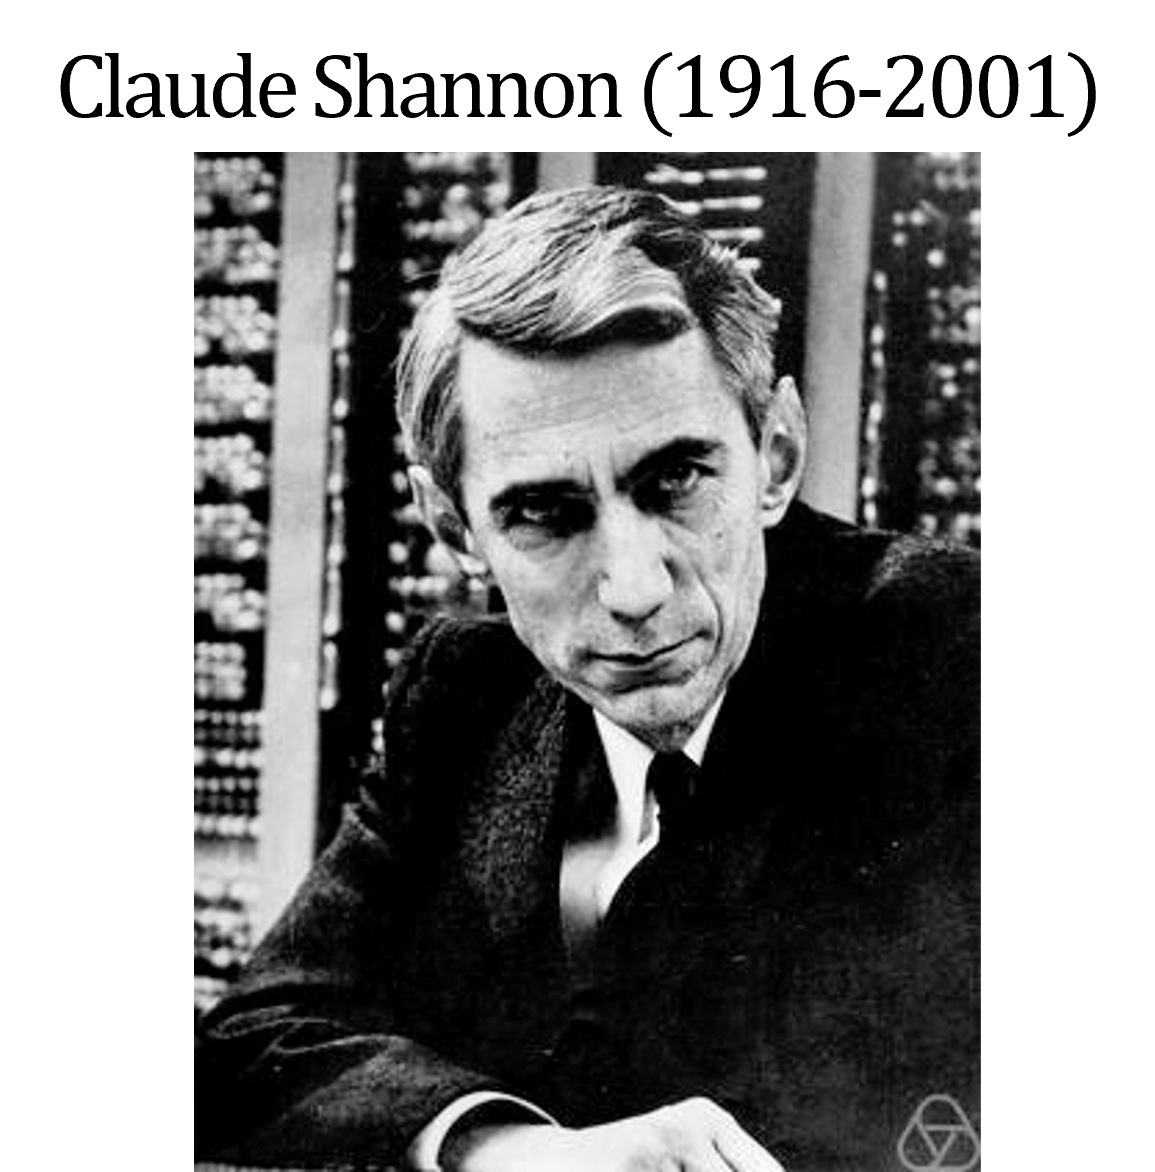
\includegraphics[width=0.6\linewidth]{figure/shannon.png}  % Adjust the width as needed
            \caption{Viste, hvordan boolesk algebra kan bruges til at konstruere computerkredsløb.}
        \end{center}
    \end{multicols}
\end{figure}

Selv om Boole lagde grunden, var det først i 1930'erne, at \textbf{Claude Shannon}, der bredt anses for informationsteoriens fader, viste, hvordan boolesk algebra kunne anvendes til at konstruere elektroniske kredsløb. I sit banebrydende speciale viste Shannon, at boolesk algebra kunne bruges til at modellere og forenkle de komplekse arrangementer af kontakter og relæer, som findes i elektriske kredsløb. Denne erkendelse slog bro mellem abstrakt matematisk logik og praktisk ingeniørarbejde og lagde grunden til de digitale kredsløb, der bruges i moderne computere. Shannons speciale vandt Alfred Noble-prisen i 1939.

\subsection*{Relevans for datalogi}
Boolesk algebra spiller en central rolle i datalogi, især i design og funktion af digitale systemer som computere, mobile enheder og indlejrede systemer. Grundlæggende bruges boolesk algebra til at modellere og designe opførslen af \textbf{digitale kredsløb}. De er bygget af elektroniske komponenter med to tilstande: tændt eller slukket, hvilket svarer direkte til de binære værdier 1 og 0.

Kernen i disse digitale kredsløb er \textbf{transistorer}. En transistor er en halvlederkomponent, der kan styre elektrisk strøm og derfor kan bruges som en elektronisk kontakt. Moderne processorer indeholder milliarder af forbundne transistorer.

\begin{figure}[h]
    \centering
    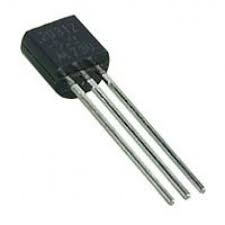
\includegraphics[width = 0.3\textwidth]{figure/transistor.png} % Adjust width here to scale the image
    \caption{En transistor.}
    \label{fig:transistor}
\end{figure}

Transistorerne kan forbindes på en sådan måde, at de gemmer information i binær form -- hvert 0 eller 1 repræsenterer en enkelt bit information. Desuden kan de bruges til at udføre logiske operationer på disse bit.

Enhver beregning eller beslutning, som en computer foretager, involverer en række logiske operationer -- såsom \texttt{AND}, \texttt{OR} og \texttt{NOT} -- der beskrives og optimeres ved hjælp af booleske udtryk. Disse logiske operationer er grundlæggende for styringen af datastrømme og beslutninger i software- og hardwaresystemer. For eksempel:

\begin{itemize}
    \item I \textbf{processorer} bruges boolesk algebra til at skabe \textbf{logiske gates} og kredsløb, der står for databehandling, regneoperationer og beslutninger.
    \item I \textbf{software} bygger betingede sætninger som \texttt{IF} og \texttt{ELSE} på boolesk logik og afgør, hvilke veje et program følger.
\end{itemize}

Ud over digitale kredsløb ligger boolesk algebra også til grund for centrale begreber inden for \textbf{logikprogrammering}, \textbf{databaseforespørgsler} og \textbf{søgealgoritmer}, hvor betingelser skal evalueres som \texttt{TRUE} eller \texttt{FALSE}.

På det fysiske niveau fungerer kredsløbene i digitale enheder ved at behandle binære input og frembringe et binært output. Hvert af disse kredsløb kan modelleres med booleske funktioner, som er udtryk, der beskriver, hvordan inputværdierne behandles for at frembringe et output. En simpel \texttt{AND}-gate giver for eksempel kun outputtet 1, hvis begge dens input er 1, hvilket svarer direkte til den booleske operation \( x \land y \).

Boolesk algebra er ikke kun en måde at forenkle logiske ræsonnementer på, men også et værktøj til at optimere design af digitale kredsløb. Ved at reducere booleske udtryk kan designere mindske antallet af nødvendige logiske gates. Det giver mere effektive kredsløb, der bruger mindre strøm og fylder mindre på en chip.

\section{Grundlæggende operationer på bit}
De booleske operatorer definerer de grundlæggende regler for behandling af binære værdier (0 og 1). De tre primære operationer i boolesk algebra er:

\begin{custombox}{Primære booleske operationer}
    

\begin{itemize}
    \item \textbf{Komplementering} (betegnes \texttt{NOT}, fx $\overline{0}$)
    \item \textbf{Boolesk sum} (betegnes \texttt{OR}, fx $1 + 0$)
    \item \textbf{Boolesk produkt} (betegnes \texttt{AND}, fx $1 \cdot 0$)
\end{itemize}
\end{custombox}

\textbf{Komplementet} af en boolesk værdi er den modsatte tilstand. Det betegnes med en streg over variablen. For eksempel:

\[
\overline{0} = 1, \quad \overline{1} = 0
\]

Komplementeringen vender værdien: Hvis input er 0, er output 1, og omvendt.

Den booleske sum, eller \texttt{OR}, er en logisk operation, der giver 1, hvis mindst én af operanderne er 1. Resultaterne er som følger:
\[
1 + 1 = 1, \quad 1 + 0 = 1, \quad 0 + 1 = 1, \quad 0 + 0 = 0
\]
Denne operation svarer til addition, men følger andre regler for binær logik.

Det booleske produkt, eller \texttt{AND}, giver kun 1, hvis begge operander er 1. Resultaterne er:
\[
1 \cdot 1 = 1, \quad 1 \cdot 0 = 0, \quad 0 \cdot 1 = 0, \quad 0 \cdot 0 = 0
\]
I nogle tilfælde kan multiplikationstegnet (\texttt{AND}) udelades for overskuelighedens skyld, på samme måde som det udelades ved multiplikation i algebra.

Vi kan opsummere overvejelserne om de grundlæggende booleske operatorer i følgende tabel:

\begin{table}[h!]
    \begin{center}
    \begin{tabular}{ccc}
    \underline{\texttt{OR}} & \underline{\texttt{AND}} & \underline{\texttt{NOT}} \\
    $0 + 0 = 0$ & $0 \cdot 0 = 0$ & $\overline{0} = 1$ \\
    $0 + 1 = 1$ & $0 \cdot 1 = 0$ & $\overline{1} = 0$ \\
    $1 + 0 = 1$ & $1 \cdot 0 = 0$ & \\
    $1 + 1 = 1$ & $1 \cdot 1 = 1$ & \\
    \end{tabular}
    \end{center}
    \caption{Grundlæggende booleske operatorer.}
    \label{tab:basicops}
\end{table}


\begin{remark} En \textbf{boolesk variabel} kan kun antage to mulige værdier: 0 (\texttt{FALSE}) eller 1 (\texttt{TRUE}). Disse variable repræsenterer tilstandene i logiske kredsløb. Givet $x = 1$ og $y = 0$ kan du for eksempel anvende booleske operationer:

\[
x + y = 1, \quad x \cdot y = 0, \quad \overline{x} = 0
\]

Vi bruger typisk $x, y$ og $z$ som vores booleske variable.

\end{remark}

\subsection*{Operatorpræcedens}
Når udtryk med flere booleske operatorer skal evalueres, anvendes følgende rækkefølge:
\begin{enumerate}
    \item Komplementer (\texttt{NOT}) evalueres først.
    \item Booleske produkter (\texttt{AND}) beregnes derefter.
    \item Booleske summer (\texttt{OR}) evalueres til sidst.
\end{enumerate}

For eksempel betyder $x \cdot y+z$ altså $(x \cdot y)+z$. I de fleste tilfælde skriver vi dog parenteserne for at undgå misforståelser. Bemærk også, at parenteser kan bruges til at tilsidesætte den normale præcedens, så bestemte operationer evalueres før andre.

Se på udtrykket:
\[
\overline{x} \cdot y + z
\]
Ifølge præcedensreglerne evalueres komplementet (\texttt{NOT}) af $x$ først, derefter det booleske produkt (\texttt{AND}) af $\overline{x}$ og $y$ og til sidst den booleske sum (\texttt{OR}) med $z$. Det kan skrives eksplicit som:
\[
(\overline{x} \cdot y) + z
\]

Se nu på et andet udtryk:
\[
\overline{x \cdot (y + z)}
\]
Her tilsidesætter parenteserne den normale præcedens. Den booleske sum (\texttt{OR}) af $y$ og $z$ evalueres først, derefter det booleske produkt (\texttt{AND}) med $x$ og til sidst komplementet (\texttt{NOT}) af hele resultatet.

\begin{example}
    Find værdien af $1 \cdot 0+\overline{(0+1)}$.

    \begin{solution}
        Ud fra definitionerne af komplementering, sum og produkt og rækkefølgen af operationerne følger det, at
        \[
        \begin{aligned}
        1 \cdot 0+\overline{(0+1)} & =0+\overline{1} \\
        & =0+0 \\
        & =0
        \end{aligned}
        \]
    \end{solution}
    \label{ex4.1}
\end{example}

Det viser sig, at de booleske operatorer er tæt forbundet med de logiske operatorer.

\subsection*{Logiske operatorer}
Komplementet, den booleske sum og det booleske produkt svarer til henholdsvis de logiske operatorer $\neg$, $\vee$ og $\wedge$. I denne sammenhæng svarer 0 til \texttt{FALSE} ($\mathbf{F}$), og 1 svarer til \texttt{TRUE} ($\mathbf{T}$). 

Ligheder i boolesk algebra kan oversættes direkte til ækvivalenser mellem sammensatte udsagn i logik. Tilsvarende kan logiske ækvivalenser oversættes til ligheder i boolesk algebra. Disse oversættelser gør det muligt at bevæge sig gnidningsløst mellem boolesk algebra og udsagnslogik.

\begin{example}
    Oversæt $1 \cdot 0+\overline{(0+1)}=0$, den lighed, vi fandt i Eksempel \ref{ex4.1}, til en logisk ækvivalens.

    \begin{solution}
        $(\mathbf{T} \wedge \mathbf{F}) \vee \neg(\mathbf{F} \vee \mathbf{T}) \equiv \mathbf{F}$
    \end{solution}
    
\end{example}

Da logik er et selvstændigt fagområde, går vi ikke videre med det her.\footnote{Symbolet »$\equiv$« betegner logisk ækvivalens: To udsagn er logisk ækvivalente, når de har samme sandhedsværdi for enhver tildeling af værdier til deres variable. Ækvivalente udsagn behøver ikke at have samme syntaktiske struktur. I boolesk algebra angiver »$=$« tilsvarende, at to booleske udtryk definerer den samme funktion for alle input.}

\section{Booleske funktioner}

En \textbf{boolesk funktion} afbilder booleske input over i et boolesk output. Se på den booleske funktion $F(x, y, z)$:

\[
F(x, y, z) = (x \cdot \overline{y}) + z
\]

Funktionen giver resultatet af boolesk \texttt{OR} mellem to led: $x \cdot \overline{y}$ (\texttt{AND} af $x$ og komplementet af $y$) og $z$. Nedenfor er funktionen vist i en tabel, som angiver værdien af $F$ for alle kombinationer af inputværdier:

\begin{table}[h!]
        \begin{center}
        \renewcommand{\arraystretch}{1.5} % Adjusts row spacing
        \begin{tabular}{c|c|c|c}
        $x$ & $y$ & $z$ & $F(x, y, z)$ \\
        \hline
        0 & 0 & 0 & 0 \\
        \rowcolor{gray!20}
        0 & 0 & 1 & 1 \\
        0 & 1 & 0 & 0 \\
        \rowcolor{gray!20}
        0 & 1 & 1 & 1 \\
        1 & 0 & 0 & 1 \\
        \rowcolor{gray!20}
        1 & 0 & 1 & 1 \\
        1 & 1 & 0 & 0 \\
        \rowcolor{gray!20}
        1 & 1 & 1 & 1 \\
        \end{tabular}
        \end{center}
    \caption{Sandhedstabel for $F(x, y, z) = (x \cdot \overline{y}) + z$.}
    \label{tab:ttexam}
\end{table}

\begin{example}Se på den booleske funktion, der er defineret ved:
    \[
F(x, y, z) = xy + \overline{z}
\]

Opstil sandhedstabellen for funktionen.

\begin{solution} Funktionen er vist i tabellen nedenfor, som angiver værdien af \( F \) for alle kombinationer af inputværdierne \( x \), \( y \) og \( z \):

\begin{table}[h!]
\begin{center}
\renewcommand{\arraystretch}{1.5} % Adjusts row spacing
\begin{tabular}{c|c|c|c|c|c}

$x$ & $y$ & $z$ & $xy$ & $\overline{z}$ & $F(x, y, z)$ \\
\hline
0 & 0 & 0 & 0 & 1 & 1 \\
\rowcolor{gray!20}
0 & 0 & 1 & 0 & 0 & 0 \\
0 & 1 & 0 & 0 & 1 & 1 \\
\rowcolor{gray!20}
0 & 1 & 1 & 0 & 0 & 0 \\
1 & 0 & 0 & 0 & 1 & 1 \\
\rowcolor{gray!20}
1 & 0 & 1 & 0 & 0 & 0 \\
1 & 1 & 0 & 1 & 1 & 1 \\
\rowcolor{gray!20}
1 & 1 & 1 & 1 & 0 & 1 \\
\end{tabular}
\end{center}
\caption{Sandhedstabel for den booleske funktion \( F(x, y, z) = xy + \overline{z} \).}
\label{tab:boolean_example}
\end{table}

Søjlerne \( xy \) og \( \overline{z} \) er »hjælpesøjler«, der hjælper med at beregne \( F \), selv om de ikke er strengt nødvendige. De opdeler udtrykket \( F(x, y, z) \) i mindre dele, så det bliver lettere at beregne det endelige resultat.
    
\end{solution}
\end{example}

\subsection*{Reduktion af et boolesk udtryk}

Tabellen nedenfor viser output for funktionerne \( F(x, y) = (x\overline{y} + xy) \cdot y \) og \( G(x, y) = xy \) for alle værdier af \( x \) og \( y \):

\begin{table}[h!]
\begin{center}
\renewcommand{\arraystretch}{1.5} % Adjust row spacing
\begin{tabular}{c|c|c|c|c|c|c|c}
$x$ & $y$ & $xy$ & $\overline{y}$ & $x\overline{y}$ & $xy + x\overline{y}$ & $F(x, y)$ & $G(x, y)$ \\
\hline
0 & 0 & 0 & 1 & 0 & 0 & 0 & 0 \\
\rowcolor{gray!20}
0 & 1 & 0 & 0 & 0 & 0 & 0 & 0 \\
1 & 0 & 0 & 1 & 1 & 1 & 0 & 0 \\
\rowcolor{gray!20}
1 & 1 & 1 & 0 & 0 & 1 & 1 & 1 \\

\end{tabular}
\end{center}
\caption{Sammenligning af \( F(x, y) = (x\overline{y} + xy) \cdot y \) og \( G(x, y) = xy \).}
\label{tab:simplifying_boolean}
\end{table}

Funktionerne giver samme output for alle værdier af \( x \) og \( y \). De to funktioner er altså ækvivalente!

Booleske udtryk kan ofte reduceres betydeligt. I det følgende afsnit ser vi nærmere på nogle regler og teknikker til at opnå denne reduktion.

\subsection*{Booleske identiteter}
Booleske identiteter er grundlæggende regler, der definerer sammenhængene og operationerne mellem booleske variable. Identiteterne gør det muligt at reducere og omskrive booleske udtryk. Ved at anvende dem kan komplekse booleske udtryk reduceres til simplere former, så de bliver lettere at evaluere eller implementere i digitale kredsløb. Uanset om der er tale om de kommutative, associative eller distributive love eller De Morgans love, er identiteterne byggestenene til effektiv logisk manipulation og hjælper os til at forstå booleske funktioners opførsel på et dybere niveau.

Vi begynder med at se på de mest grundlæggende af disse identiteter:

\begin{custombox}{Grundlæggende booleske egenskaber}
\begin{itemize}
    \item \textbf{Dobbelt komplement:} \\
    \hspace*{15pt} $\overline{\overline{x}} = x$\hspace{15pt}
    
    \item \textbf{Idempotenslove:} \\
    \hspace*{15pt}$x + x = x$, \quad $x \cdot x = x$
    
    \item \textbf{Identitetslove:} \\
    \hspace*{15pt}$x + 0 = x$, \quad $x \cdot 1 = x$
    
    \item \textbf{Dominanslove:} \\
    \hspace*{15pt}$x + 1 = 1$, \quad $x \cdot 0 = 0$
    
    \item \textbf{Enhedsegenskaben:} \\
    \hspace*{15pt}$\overline{x} + x = 1$
    
    \item \textbf{Nulegenskaben:} \\
    \hspace*{15pt} $\overline{x} \cdot x = 0$
\end{itemize}
\end{custombox}

Disse identiteter udgør de mest grundlæggende egenskaber ved boolesk algebra og handler om, hvordan \texttt{OR}, \texttt{AND} og de neutrale elementer (0 og 1) opfører sig.

\begin{example} Vis, at $(1 \cdot 1)+(\overline{0 \cdot 1}+0)=1$.         
\end{example}


\begin{solution}
    For at vise, at $(1 \cdot 1)+(\overline{0 \cdot 1}+0)=1$, deler vi udtrykket op og reducerer det trin for trin ved hjælp af booleske identiteter.

    \begin{itemize}
        \item \textbf{Trin 1:} Reducér den første del $(1 \cdot 1)$
                Ved hjælp af idempotensloven $(x \cdot x=x)$ eller ved blot at beregne resultatet:
                
                \[
                1 \cdot 1=1
                \]
                
                
                Udtrykket bliver altså:
                
                \[
                1+(\overline{0 \cdot 1}+0)
                \]
        \item \textbf{Trin 2:} Reducér den anden del $(\overline{0 \cdot 1}+0)$
                Reducér først $0 \cdot 1$ ved hjælp af dominansloven $(0 \cdot x=0)$:
                
                \[
                0 \cdot 1=0
                \]
                
                
                Udtrykket bliver altså:
                
                \[
                1+(\overline{0}+0)
                \]
        \item \textbf{Trin 3:} Reducér komplementet $\overline{0}$
    Ved hjælp af komplementloven $(\overline{0}=1)$:
    
    \[
    \overline{0}=1
    \]

    
    
    Dermed bliver udtrykket:
    
    \[
    1+(1+0)
    \]

    \item \textbf{Trin 4:} Reducér det indre udtryk \( (1 + 0) \) \\
        Ved hjælp af identitetsloven \( (x + 0 = x) \):
        
        \[
        1 + 0 = 1
        \]
        
        Udtrykket bliver nu:
        
        \[
        1 + 1
        \]
        
        \item \textbf{Trin 5: }Reducér \( 1 + 1 \) \\
        Ved hjælp af idempotensloven \( (x + x = x) \) eller dominansloven:
        
        \[
        1 + 1 = 1
        \]
        
        Udtrykket er sandt. \end{itemize}
        Dermed har vi vist, at:
        
        \[
        (1 \cdot 1) + (\overline{0 \cdot 1} + 0) = 1
        \]
        \end{solution}

Dernæst ser vi på nogle andre vigtige love:

\begin{custombox}{Strukturelle booleske love}
\begin{itemize}
    \item \textbf{Kommutative love:} \\
    \hspace*{15pt}$x + y = y + x$, \quad $x \cdot y = y \cdot x$
    
    \item \textbf{Absorptionslove og beslægtede forenklingsregler:} \\
    \hspace*{15pt}$x + (x \cdot y) = x$, \quad $x \cdot (x + y) = x$, \quad $\bar{x} \cdot \bar{y}+x=\bar{y}+x$
    
    \item \textbf{De Morgans love:} \\
    \hspace*{15pt} $\overline{x \cdot y} = \overline{x} + \overline{y}$, \quad $\overline{x + y} = \overline{x} \cdot \overline{y}$
    \item \textbf{Associative love:} \\
    \hspace*{15pt} $x + (y + z) = (x + y) + z$, \quad $x \cdot (y \cdot z) = (x \cdot y) \cdot z$
    
    \item \textbf{Den distributive lov:} \\
    \hspace*{15pt} $x \cdot (y + z) = (x \cdot y) + (x \cdot z)$, \quad $x + (y \cdot z) = (x + y) \cdot (x + z)$
\end{itemize}
\end{custombox}

Sammen med de grundlæggende identiteter gør de strukturelle love det muligt at reducere mere komplekse udtryk.

\begin{example}
    Vis, at
    \(
    (x \cdot y) + \overline{(x + z) \cdot \overline{y}} = y + \overline{x} \cdot \overline{z}
    \)
\end{example}

\begin{solution}

    Bemærk, at vi ikke eksplicit nævner brugen af de \textbf{kommutative love}.

    \begin{itemize}

        \item \textbf{Trin 1:} Anvend \textbf{De Morgans lov} på komplementet
        
        \[ \overline{(x + z) \cdot \overline{y}} \]
        
        Udtrykket bliver:
        
        \[
        (x \cdot y) + \overline{(x + z)} + \overline{\overline{y}}
        \]
        
        \item \textbf{Trin 2:} Brug \textbf{loven om dobbelt komplement}
        
        \[
        \overline{\overline{y}}
        \]
        
        Udtrykket bliver:

         \[
        (x \cdot y) + \overline{(x + z)} + y
        \]
        
        \item \textbf{Trin 3:} Anvend \textbf{De Morgans lov} på komplementet
             
        \[
        \overline{(x + z)}
        \]
        
        Udtrykket bliver:

        \[
       (x \cdot y) + \overline{x} \cdot \overline{z} + y
       \]
        
        \item \textbf{Trin 4:} Anvend \textbf{den distributive lov} baglæns
        
        \[
        (x \cdot y) + \overline{x} \cdot \overline{z} + y = y (x + 1) + \overline{x} \cdot \overline{z}
        \]
        
        \item \textbf{Trin 5:} Brug \textbf{dominansloven} til at reducere \( x + 1 \):
        
        Udtrykket reduceres altså til:
        
        \[
        y + \overline{x} \cdot \overline{z}
        \]
        
    \end{itemize}
    
    Dermed har vi vist, at:
    
    \[
    (x \cdot y) + \overline{(x + z) \cdot \overline{y}} = y + \overline{x} \cdot \overline{z}
    \]
    

\end{solution}

Ud over de grundlæggende operatorer har vi andre almindeligt anvendte operatorer i boolesk algebra:

\begin{itemize}
\setlength{\itemsep}{10pt}
    \item \texttt{NOT} \texttt{AND} (\texttt{NAND}): Dette er komplementet til \texttt{AND}-operationen. Den giver sand, medmindre begge input er sande. I boolesk algebra betegnes \texttt{NAND} med symbolet $\uparrow$ og kan skrives som: \[
        x \uparrow y = \overline{x \cdot y}
        \]

    \item \texttt{NOT} \texttt{OR} (\texttt{NOR}): Operatoren \texttt{NOR} er komplementet til \texttt{OR}-operationen. Den giver kun sand, når begge input er falske. Den betegnes med symbolet $\downarrow$ og kan udtrykkes som:
        \[
        x \downarrow y = \overline{x + y}
        \]

    \item Eksklusiv \texttt{OR} (\texttt{XOR}): Operatoren \texttt{XOR} giver sand, hvis præcis ét af input er sandt, men ikke begge. Det er særligt nyttigt i regneoperationer som binær addition. Den betegnes med $\oplus$, og det booleske udtryk for \texttt{XOR} er:
        \[
        x \oplus y = (x \cdot \overline{y}) + (\overline{x} \cdot y)
        \]

\end{itemize}

Vi opsummerer de supplerende operatorer i følgende tabel:

\begin{table}[h!]
\begin{center}
\begin{tabular}{ccc}
\underline{\texttt{NAND}} & \underline{\texttt{NOR}} & \underline{\texttt{XOR}} \\
$0 \uparrow 0 = 1$ & $0 \downarrow 0 = 1$ & $0 \oplus 0 = 0$ \\
$0 \uparrow 1 = 1$ & $0 \downarrow 1 = 0$ & $0 \oplus 1 = 1$ \\
$1 \uparrow 0 = 1$ & $1 \downarrow 0 = 0$ & $1 \oplus 0 = 1$ \\
$1 \uparrow 1 = 0$ & $1 \downarrow 1 = 0$ & $1 \oplus 1 = 0$ \\
\end{tabular}
\end{center}
    \caption{Supplerende booleske operatorer.}
    \label{tab:addibool}
\end{table}


Her er alle operatorerne samlet i én tabel:

\begin{table}[h!]
    \begin{center}
    \renewcommand{\arraystretch}{1.5} % Adjust this value for desired spacing
    \begin{tabular}{c|c|c|c|c|c}
    \texttt{OR} & \texttt{AND} & \texttt{NOT} & \texttt{NAND} & \texttt{NOR} & \texttt{XOR} \\
    \hline % Keeps one horizontal line below the operator names
    $0 + 0 = 0$ & $0 \cdot 0 = 0$ & $\overline{0} = 1$ & $0 \uparrow 0 = 1$ & $0 \downarrow 0 = 1$ & $0 \oplus 0 = 0$ \\
    $0 + 1 = 1$ & $0 \cdot 1 = 0$ & $\overline{1} = 0$ & $0 \uparrow 1 = 1$ & $0 \downarrow 1 = 0$ & $0 \oplus 1 = 1$ \\
    $1 + 0 = 1$ & $1 \cdot 0 = 0$ & & $1 \uparrow 0 = 1$ & $1 \downarrow 0 = 0$ & $1 \oplus 0 = 1$ \\
    $1 + 1 = 1$ & $1 \cdot 1 = 1$ & & $1 \uparrow 1 = 0$ & $1 \downarrow 1 = 0$ & $1 \oplus 1 = 0$ \\
    \end{tabular}
    \end{center}
    \caption{Grundlæggende og supplerende booleske operatorer.}
    \label{tab:mergedops}
\end{table}


Nu kan vi angive de sidste og mere avancerede booleske identiteter:

\begin{custombox}{Avancerede booleske identiteter}
\begin{itemize}
    \item \textbf{Eksklusiv \texttt{OR} (\texttt{XOR}):} \\
    \hspace*{15pt} $x \oplus y = (x \cdot \overline{y}) + (\overline{x} \cdot y)$
    
    \item \textbf{Eksklusiv \texttt{NOR} (\texttt{XNOR}):} \\
    \hspace*{15pt} $\overline{x \oplus y} = (x \cdot y) + (\overline{x} \cdot \overline{y})$
    
    \item \textbf{Den forsvindende modsætning:} \\
    \hspace*{15pt} $x + \overline{x} \cdot y = x + y$
    
    \item \textbf{FOIL-loven (af engelsk \emph{First, Outer, Inner, Last}: første, yderste, inderste, sidste):} \\
    \hspace*{15pt} $(x + y) \cdot (z + w) = (x \cdot z) + (x \cdot w) + (y \cdot z) + (y \cdot w)$
\end{itemize}
\end{custombox}

\section{Logiske gates}
Logiske gates er de grundlæggende byggesten i digitale kredsløb og styrer den elektriske strøm, der løber ind i og ud af kredsløbene. Logiske gates modtager binære input og frembringer output og regulerer derved elektriske signaler. Disse gates er opbygget af transistorer og indgår også i større systemer som regneenheder, multipleksere og mikroprocessorer og muliggør vigtige elektroniske logiske operationer.

\subsubsection*{Typer af logiske gates}
Der findes forskellige logiske gates, som fungerer forskelligt afhængigt af, hvilken type binært input de modtager. I boolesk algebra svarer disse gates til grundlæggende logiske operationer som \texttt{AND}, \texttt{OR} og \texttt{NOT}. Nedenfor ses de mest almindelige typer logiske gates, som findes i de fleste elektroniske kredsløb:

\begin{itemize}
    \item \texttt{AND}
    \item \texttt{OR}
    \item \texttt{NOT}
    \item \texttt{NOR}
    \item \texttt{XOR}
    \item \texttt{NAND}    
\end{itemize}

Om hver af disse logiske gates aktiveres, afhænger af, om et bestemt binært input, som gaten er designet til at genkende, er til stede eller ej. Hvis inputtet passer til gatens konfiguration, giver den logiske gate outputtet 1; hvis det ikke passer, er outputtet 0.

\textbf{\texttt{AND}-gates}\\
En \texttt{AND}-gate fungerer efter alt-eller-intet-princippet. For at aktivere gaten skal alle input være 1. Hvis blot ét input er 0, bliver outputtet 0.

\textbf{\texttt{OR}-gates}\\
\texttt{OR}-gates er mindre restriktive end \texttt{AND}-gates. Hvis mindst ét input er 1, bliver outputtet 1, uanset de øvrige input.

\textbf{\texttt{NOT}-gates}\\
En \texttt{NOT}-gate inverterer sit input. Den har ét input og ét output, og outputtet er altid det modsatte af inputtet. Hvis inputtet for eksempel er 1, bliver outputtet 0, og omvendt.

\begin{figure}[h!]
    \centering
    \resizebox{0.8\textwidth}{!}{% Danish version of the overview of common logic gates (standard ANSI symbols).
\begin{circuitikz}[font=\small]
  \def\gate#1#2#3#4#5#6{% x, y, port type, symbol text, output label, caption
    \node[#3 port, anchor=center, scale=1.3] (g) at (#1,#2) {};
    \path (g.west) -- (g.east) node[midway, font=\scriptsize\sffamily] {#4};
    \draw[-{Stealth[length=5pt]}] (#1-1.9,#2 |- g.in 1) node[left, text=cyan!60!black] {$x$} -- (g.in 1);
    \draw[-{Stealth[length=5pt]}] (#1-1.9,#2 |- g.in 2) node[left, text=cyan!60!black] {$y$} -- (g.in 2);
    \draw[-{Stealth[length=5pt]}] (g.out) -- (#1+1.9,#2 |- g.out) node[pos=0.5, above, text=cyan!60!black] {#5};
    \node[anchor=north] at (#1,#2-0.85) {#6};
  }
  \node[not port, anchor=center, scale=1.3] (n) at (0,0) {};
  \draw[-{Stealth[length=5pt]}] (-1.9,0 |- n.in) node[left, text=cyan!60!black] {$x$} -- (n.in);
  \draw[-{Stealth[length=5pt]}] (n.out) -- (1.9,0 |- n.out) node[pos=0.5, above, text=cyan!60!black] {$\bar{x}$};
  \node[anchor=north] at (0,-0.85) {NOT-gate};
  \gate{5.5}{0}{or}{OR}{$x + y$}{OR-gate}
  \gate{11}{0}{and}{AND}{$xy$}{AND-gate}
  \gate{0}{-3}{nand}{NAND}{$x \uparrow y$}{NAND-gate}
  \gate{5.5}{-3}{nor}{NOR}{$x \downarrow y$}{NOR-gate}
  \gate{11}{-3}{xor}{XOR}{$x \oplus y$}{XOR-gate}
\end{circuitikz}
}
    \caption{ANSI-symboler for de mest almindelige logiske gates. (\cite{rosen2012}).}
    \label{fig:gates}
\end{figure}

\textbf{\texttt{NOR}-gates}\\
En \texttt{NOR}-gate kombinerer egenskaberne ved en \texttt{OR}-gate med en inverter. Outputtet fra en \texttt{NOR}-gate er kun 1, når alle input er 0. Alle andre kombinationer af input giver outputtet 0.

\textbf{\texttt{XOR}-gates}\\
En \texttt{XOR}-gate (eksklusiv OR) giver kun outputtet 1, når præcis ét af dens input er 1. Hvis begge input er ens, enten begge 0 eller begge 1, bliver outputtet 0. Den fungerer som en \texttt{OR}-gate, men med den ekstra betingelse, at begge input ikke samtidig må være 1, for at den giver 1.

\textbf{\texttt{NAND}-gates}\\
En \texttt{NAND}-gate er en kombination af en \texttt{AND}-gate og en \texttt{NOT}-gate. Outputtet er kun 0, hvis alle input er 1. I alle andre tilfælde er outputtet 1.

På samme måde som vi tidligere reducerede booleske udtryk til simplere former, kan vi opnå samme output med forskellige kredsløbsdesign, som det ses i figur \ref{fig:gates2}.

\begin{figure}[h!]
    \centering
    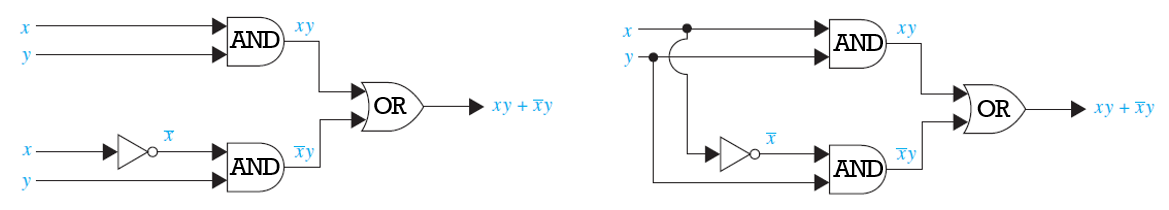
\includegraphics[width = 0.9\textwidth]{figure/gatessimilar.png} % Adjust width here to scale the image
    \caption{To ækvivalente kredsløb af logiske gates. (\cite{rosen2012}).}
    \label{fig:gates2}
\end{figure}

Vi afslutter kapitlet med at se på idéen om \textbf{funktionel fuldstændighed}, også kendt som en \textbf{universel gate}. Begrebet henviser til en mængde af logiske gates, der kan kombineres, så de implementerer en vilkårlig boolesk funktion. En funktionelt fuldstændig mængde af gates, såsom \texttt{NAND} eller \texttt{NOR}, kan altså efterligne opførslen af alle de andre grundlæggende logiske gates, hvilket gør dem til alsidige værktøjer i design af digitale kredsløb.


\subsubsection*{Funktionel fuldstændighed og universelle gates}
En operator eller en mængde af operatorer kaldes \textbf{funktionelt fuldstændig}, hvis den kan bruges til at udtrykke en vilkårlig boolesk funktion. Både \texttt{NAND}- og \texttt{NOR}-gates er funktionelt fuldstændige, eller \textbf{universelle gates}. Det betyder, at ethvert logisk udtryk kan konstrueres med kun \texttt{NAND} eller kun \texttt{NOR}.

Grunden til, at \texttt{NAND}-gaten (eller \texttt{NOR}-gaten) er funktionelt fuldstændig, er dens evne til at efterligne andre booleske operationer. Med \texttt{NAND}-operationer alene kan vi konstruere de grundlæggende operationer \texttt{NOT}, \texttt{AND} og \texttt{OR}, som er byggestenene i enhver boolesk funktion.

\begin{itemize}
\setlength{\itemsep}{10pt}
    \item \texttt{NOT} (\(\overline{x}\)): En \texttt{NOT}-gate kan konstrueres ved at forbinde begge input på en \texttt{NAND}-gate til den samme variabel:
    \(
    \overline{x} = x \uparrow x
    \)

    \item \texttt{AND} (\(x \cdot y\)): \texttt{AND}-operationen kan opnås ved først at anvende en \texttt{NAND}-gate og derefter sende resultatet gennem en \texttt{NOT} (som, vi har set, også kan konstrueres med \texttt{NAND}): \newline
   $x \cdot y=\overline{x \uparrow y}=(x \uparrow y) \uparrow(x \uparrow y)$

    \item \texttt{OR} (\(x + y\)): \texttt{OR}-operationen kan dannes med flere \texttt{NAND}-gates ved at udnytte De Morgans love:
    \(
    x + y = (x \uparrow x) \uparrow (y \uparrow y)
    \)
\end{itemize}


Tabellen nedenfor viser, hvordan vi kan konstruere de grundlæggende booleske operationer med kun \texttt{NAND}-gates. Læg mærke til, hvordan de forskellige søjler viser transformationer af variablene $x$ og $y$, hvor kombinationer af \texttt{NAND}-gates danner de logiske operationer \texttt{NOT}, \texttt{AND} og \texttt{OR}:

\begin{table}[h!]
    \begin{center}
    \renewcommand{\arraystretch}{1.5} % Adjust this value for desired spacing
    \begin{tabular}{|c|c|c|c|c|}
    \textbf{Input} & \textbf{Input} & \textbf{NOT} & \textbf{AND} & \textbf{OR} \\
    $x$ & $y$ & $x \uparrow x$ & $(x \uparrow y) \uparrow (x \uparrow y)$ & $(x \uparrow x) \uparrow (y \uparrow y)$ \\
    \hline
    0 & 0 & 1 & 0 & 0 \\
    0 & 1 & 1 & 0 & 1 \\
    1 & 0 & 0 & 0 & 1 \\
    1 & 1 & 0 & 1 & 1 \\
    \end{tabular}
    \end{center}
    \caption{Konstruktion af grundlæggende booleske operatorer med \texttt{NAND}-gates.}
\end{table}

Da vi har set, hvordan alle booleske funktioner kan bygges med kun \texttt{NAND}-gates, forstår vi nu, at alle logiske operationer i en computer kan implementeres med denne ene type gate. Det gør \texttt{NAND}-gaten utrolig vigtig i design af digitale kredsløb, da den giver mulighed for simplere og mere effektiv implementering i hardware. I moderne computersystemer bruges transistorer til at bygge \texttt{NAND}-gates, hvilket betyder, at enhver logisk operation i sidste ende kan repræsenteres ved en kombination af transistorer.

\begin{figure}[h!]
    \centering
    \DaLogicInComp{width = 0.9\textwidth}
    \caption{Logiske gates i computere.}
    \label{fig:logincom}
\end{figure}

Begrebet funktionel fuldstændighed er således ikke kun teoretisk; det er et stærkt princip, der gør det muligt for computeringeniører at designe fleksible og effektive kredsløb med et minimum af komponenter.
